%<dscrpt>Fonctions harmoniques discrètes.</dscrpt>
Dans ce problème, on considère l'ensemble $\Z^2 = \Z\times \Z$. On pourra aussi utiliser le mot \emph{point} pour désigner un élément de $\Z^2$.\newline
Les fonctions $x$ et $y$ sont définies dans $\Z^2$ et à valeurs dans $\Z$ par:
\begin{displaymath}
  \forall c\in \Z^2, \; c=(x(c),y(c))
\end{displaymath}
On définit une relation $\mathcal{C}$ (dite de \emph{contiguïté}) dans $\Z^2$ par:
\begin{displaymath}
  \forall (c,c')\in \Z^2 \times \Z^2, c \,\mathcal{C}\, c' \Leftrightarrow (x(c')-x(c))^2 + (y(c')-y(c))^2 = 1
 \end{displaymath}
Lorsque $c \,\mathcal{C}\, c'$ est vraie, on dit que $c'$ est contigu à $c$. On note $\mathcal{V}(c)$ l'ensemble des points contigus à $c$ (voisinage de $c$).\newline
Dans tout le problème, $\Omega$ désigne une partie non vide \emph{finie} de $\Z^2$. on note $C(\Omega)$ le complémentaire de $\Omega$ dans $\Z^2$. On adopte les définitions suivantes pour les points de $c\in\Omega$.
\begin{itemize}
  \item $c$ est \emph{sur la frontière} de $\Omega$ si et seulement si il est contigu à un point de $C(\Omega)$.\newline On note $Fr(\Omega)$ l'ensemble des points sur la frontière de $\Omega$.
  \item $c$ est \emph{intérieur} à $\Omega$ si et seulement si il n'est pas sur la frontière de $\Omega$.\newline On note $\overset{\circ}{\Omega}$ l'ensemble des points intérieurs à $\Omega$.
\end{itemize}
On définit aussi une fonction $n$ de $\overset{\circ}{\Omega}$ dans $\N$ par:
\begin{displaymath}
  \forall c \in \overset{\circ}{\Omega},\;n(c) = \text{nombre de points de $Fr(\Omega)$ contigus à $c$}
\end{displaymath}
On dira enfin, pour tout point $c$ intérieur ($c\in \overset{\circ}{\Omega}$) que:
\begin{itemize}
  \item $c$ est une \emph{pointe} de $\overset{\circ}{\Omega}$ si et seulement si $n(c) = 3$,
  \item $c$ est un \emph{coin} de $\overset{\circ}{\Omega}$ si et seulement si $n(c) = 2$.
  \item $c$ est un \emph{bord} de $\overset{\circ}{\Omega}$ si et seulement si $n(c) = 1$.
\end{itemize}


\subsection*{Partie 1. Vocabulaire.}
\begin{enumerate}
  \item
\begin{enumerate}
  \item  La relation de contiguïté est-elle réflexive? symétrique? antisymétrique? transitive?
  \item Soit $c=(a,b)\in \Z^2$, préciser l'ensemble $\mathcal{V}(c)$. Combien contient-il d'éléments?
  \item Soit $c\in \Omega$, formuler avec des quantificateurs la phrase $c\in Fr(\Omega)$; même question avec $c\in \overset{\circ}{\Omega}$. Caractériser $c\in \overset{\circ}{\Omega}$ par une relation ensembliste contenant une intersection puis par une relation ensembliste contenant une inclusion.
\end{enumerate}
\begin{figure}[h]
  \centering
  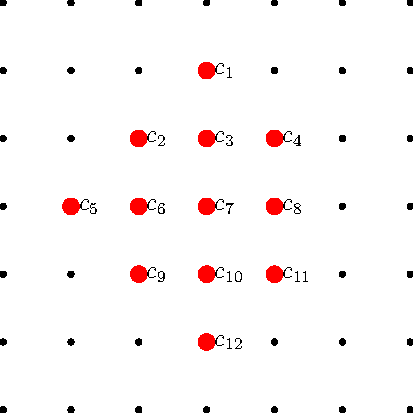
\includegraphics{./Eharmonic_1.pdf}
  \caption{Exemple de partie $\Omega$.}
  \label{fig: harmonic_1}
\end{figure}

\item Sur l'exemple de la figure \ref{fig: harmonic_1}, préciser la frontière et l'intérieur de $\Omega$, expliciter la fonction $n$. Qui sont les bords, les coins, les pointes?

\item Soit $c=(a,b)\in \Z^2$. Calculer la moyenne des valeurs prises par la fonction $x^2$ sur les points contigus à $c$, même question pour la fonction $xy$.
\end{enumerate}

\subsection*{Partie 2. Fonctions harmoniques discrètes.}
Une fonction $f$ définie sur une partie finie $\Omega$ de $\Z^2$ et à valeurs complexes est dite \emph{harmonique discrète} si et seulement si, pour chaque $c$ dans l'intérieur de $\Omega$, la valeur $f(c)$ est la moyenne des valeurs de $f$ aux points contigus à $c$.\newline
Pour certaines parties $\Omega$, une fonction arbitraire définie seulement sur la frontière admet un unique prolongement harmonique à $\Omega$ tout entier.\newline
On identifie ici $\Z^2$ à l'ensemble des complexes dont les parties réelles et imaginaires sont des entiers. On se donne une partie $\Omega={c_1,c_2,\cdots, c_{10}}$ par un tableau en précisant $c_1=0$ (donc $c_7 = 1+i, \cdots$ )
\begin{center}
\begin{tabular}{llllll}
$.$&$.$ & $.$ & $.$ & $.$ & $.$\\
$.$&$.$ & $.$ & $c_8$ & $.$ & $.$\\
$.$&$.$ & $c_9$ & $c_2$ & $c_7$ & $.$\\
$.$&$c_{10}$ & $c_3$ & $c_1$ & $c_6$ & $.$\\
$.$&$.$ & $c_4$ & $c_5$ & $.$ & $.$\\
$.$&$.$ & $.$ & $.$ & $.$ & $.$
\end{tabular}
\end{center}
\begin{enumerate}
  \item Préciser la frontière et l'intérieur de $\Omega$.
  \item Pour une fonction $f$ quelconque de $\Omega$ dans $\C$, on note
  \begin{displaymath}
f(c_i)=    \left\lbrace 
    \begin{aligned}
      &f_i \text{ si } c_i \in Fr(\Omega)\\
      &y_i \text{ si } c_i \in \overset{\circ}{\Omega}
    \end{aligned}
\right. 
  \end{displaymath}
\begin{enumerate}
  \item Former un système $(\mathcal{S})$ d'équations linéaires d'inconnues $x_1,\cdots$ (à préciser) et caractériser le fait que $f$ soit harmonique à l'aide de ce système.
  \item Montrer que si on se donne une fonction arbitraire sur la frontière de $\Omega$, on peut la prolonger de manière unique en une fonction harmonique discrète sur $\Omega$. (Utiliser uniquement des opérations élémentaires et les coder précisement)
\end{enumerate}
\item Pour une fonction $f$ définie sur la frontière par 
\begin{displaymath}
  \forall c\in Fr(\Omega),\; f(c) = c^2
\end{displaymath}
Présenter dans un tableau les valeurs de $f$ sur la frontière, former le système et calculer le prolongement harmonique. Que vérifie-t-on?
\item Pour une fonction $f$ définie sur la frontière par 
\begin{displaymath}
  \forall c\in Fr(\Omega),\; f(c) = \frac{1}{c}
\end{displaymath}
Présenter dans un tableau les valeurs de $f$ sur la frontière, former le système sans le résoudre. Que peut-on dire de l'unique prolongement harmonique ?

\item Pour une partie $\Omega$ de $\Z^2$, on note $\mathcal{H}(\Omega,\C)$ l'ensemble des fonctions de $\Omega$ dans $\C$ qui sont harmoniques discrètes.
\begin{enumerate}
  \item Montrer que toute fonction constante définie dans $\Omega$ appartient à $\mathcal{H}(\Omega,\C)$. Montrer que les restrictions à $\Omega$ des fonctions $x$ et $y$ sont dans $\mathcal{H}(\Omega,\C)$.
  \item Soit $f$ et $g$ dans $\mathcal{H}(\Omega,\C)$ et $\lambda$, $\mu$ dans $\C$, montrer que $\lambda f + \mu g$ est dans $\mathcal{H}(\Omega,\C)$.
  \item Parmi les fonctions $x^2$, $y^2$, $xy$, $x^2 - y^2$, quelles sont les fonctions harmoniques ?
\end{enumerate}
\end{enumerate}
